\documentclass[a4paper,12pt]{report}
\usepackage[T1]{fontenc}
\usepackage[utf8]{inputenc}
\usepackage[italian]{babel}
\usepackage{microtype}
\usepackage{lmodern}
\pagestyle{headings}
\usepackage[italian]{varioref}
%\renewcommand{\thefootnote}{\fnsymbol{footnote}}
\usepackage{float}
\usepackage{booktabs}
\usepackage{caption}
\captionsetup{tableposition=top,figureposition=bottom,font=small,format=hang,labelfont={sf,bf}}
\usepackage{graphicx}
\usepackage{rotating}
\usepackage{amsmath}
\usepackage{url}
\usepackage{hyperref}
\hypersetup{hidelinks}
\usepackage{eurosym}

\begin{document}
	
	%%%%%%%%%%%%%%%%%%
	%%% First page %%%
	%%%%%%%%%%%%%%%%%%
	
	\begin{titlepage}
		\begin{figure}
			\vspace{-1cm}
			\centering
			
\includegraphics[scale=0.8]{image/logo.jpg}\\[1cm]
		\end{figure}
		
		\begin{center}
			{\large  \textsc{Dipartimento di Ingegneria Elettrica e delle Tecnologie dell'Informazione}}\\[0.5cm]
			{\large  \textsc{Laurea Magistrale di Ingegneria Informatica}}\\[0.5cm]
			{\large  \textsc{Corso di Big Data Analytics and Business Intelligence}}\\[1cm]
		\end{center}
		\begin{center}
			\bfseries\Huge\sc Expert Finding\\[0.3cm]\normalsize\sc Identificazione utenti con conoscenza su un dato tema\\ 
		\end{center}
		
		
		\begin{figure}[H]
			\centering
			
\includegraphics[]{image/filigrana.png}
		\end{figure}
		
		
		\vspace{-1.5cm}
		\begin{minipage}{0.4\textwidth}
			\begin{flushleft} \large
				\emph{Autori:}\\
				Davide  \textsc{Lauretano \\}\textsc{M63000792}\\ Michele  \textsc{Pommella} \\ \textsc{M63000790}\\Davide  \textsc{Trimaldi \\}\textsc{M63000799}
			\end{flushleft}
		\end{minipage}
		~
		\begin{minipage}{0.4\textwidth}
			\begin{flushright} \large
				\emph{Professore:} \\
				Antonio  \textsc{Picariello \\}
			\end{flushright}
		\end{minipage}\\
		\begin{center}
			\vfill
			{\sc Anno Accademico 2018-2019}
		\end{center}
	\end{titlepage}
	
	%%%%%%%%%%%%%%%%%%%%%%%%%%%%%
	%%% Non-significant pages %%%
	%%%%%%%%%%%%%%%%%%%%%%%%%%%%%
	
	
	\tableofcontents
	\listoffigures
	\listoftables
	
	\chapter{Problema}
La ricerca di esperti è una sfida per molte ragioni, tra cui:
\begin{itemize}
	\item Il volume di pubblicazioni di un esperto non è indice di esperienza;
	\item Il primo esperto che hai trovato potrebbe non essere il migliore;
	\item Alcuni argomenti generano più opinioni che fatti e quindi trovare il vero esperto può essere difficile;
	\item Di solito c'è una mancanza di accesso alle informazioni sulle prestazioni passate dell' esperto;
	\item Le competenze non sono distribuite in modo uniforme e punti di forza delle associazioni tra esperti variare in modo significativo
	\item Non ci sono standard che specificano i criteri e/o le qualifiche necessarie per particolari livelli di esperienza.
	\item La vera esperienza è rara e costosa. Spesso l'accesso è controllato, in modo informale o formalmente, dall'esperto stesso o dal loro management.
	\item La competenza di un esperto cambia continuamente e richiede consapevolezza di questa dinamica. 
	\item Le soluzioni a problemi complessi spesso richiedono o comunità di esperti o diverse gamme di competenze che devono essere riunite per risolvere il complesso i problemi.
	\item  Gli ingegneri di uno studio classico hanno trascorso il 16\% del loro tempo a comunicare esperti - ma la comunicazione è stata ostacolata da differenze geografiche, di fuso orario e barriere culturali.
\end{itemize}
In sintesi, la ricerca di esperti è un compito complesso e difficile.
	
	\chapter{Metodologia ed architettura}
La metodologia adoperata fa uso di un database \emph{NoSQL}, per il mantenimento dei dati, e della tecnologia \emph{Apache Spark} su macchina virtuale \emph{Azure}.\par 
La macchina virtuale mette a disponizione:
\begin{itemize}
	\item 8 core
	\item Memoria centrale di 58 GB
	\item Memoria di massa di 30 GB
	\item Disco temporaneo secondario di 350 GB
\end{itemize}
Accessibile mediante protocollo SSH, offre l'utilizzo dell'engine Apache Spark con stack relativo già installato e configurato. In particolare si è fatto uso del modello di programmazione Spark per il linguaggio Python: \emph{Pyspark}.\par
\section{MongoDB}
Il database NoSQL utilizzato è \emph{MongoDB} per la tipologia di dati da trattare e le operazioni da effettuare su di essi. MongoDB è un database documentale che consente di trattare aggregati strutturati, risultando in accesso più flessibili. Permette, quindi, di sottomettere query basate sui campi dell'aggregato e recuperare solo parte di esso. MongoDB memorizza e restituisce documenti in formato \emph{BSON}, rappresentazione binaria del JSON. I documenti sono strutture dati ad albero gerarchiche e possono essere anche strutturalmente non identici. Sono infatti distinti per collezione, insieme di documenti simili. Le caratteristiche di MongoDB hanno consentito una gestione semplice ed efficace del dataset composto principalmente da file \emph{JSON} e \emph{XML}. Il flessibile modello documentale dei dati con schema dinamico e ridimensionamento automatico su hardware comune rende MongoDB ideale per applicazioni con grandi volumi di dati multi-strutturati e dall'elevato tasso di cambiamento. Inoltre MongoDB offre la completa interoperabilità con il sistema Spark, mediante il \emph{MongoDB Spark Connector}, che ne consente la gestione tramite codice Pyspark.

\begin{figure}[H]
	\centering
	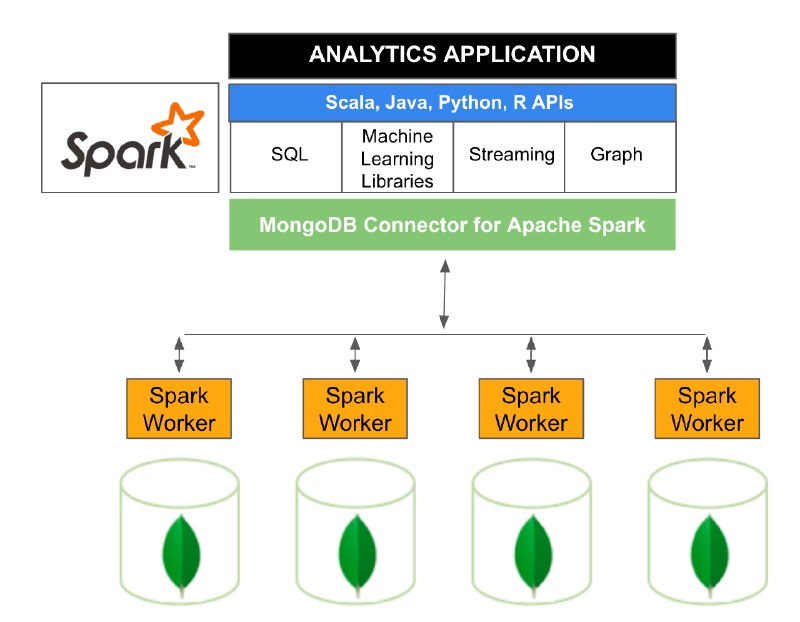
\includegraphics[scale=0.5]{image/mongospark.jpg}
	\caption{MongoDB Spark Connector}
	\label{fig:msc}
\end{figure}

\section{Spark}
Apache Spark è un framework di data processing che consente di effettuare query veloci grazie alla memorizzazione \emph{in-memory} dei dati. Supporta diversi linguaggi di programmazione: Scala, Java, R, Python. Le sue principali caratteristiche sono:
\begin{description}
	\item[Velocità] sfruttando le ottimizzazioni in-memory;
	\item[Framework unificato] offrendo packages di librerie di alto livello (supporto a query SQL, Machine Learning, stream e graph processing);
	\item[Semplicità] includendo API facili da usare per operare su grandi dataset, come operatori per trasformare e manipolare dati semistrutturati.
\end{description}
Spark, combinato con Python, è stato sfruttato sia per il caricamento del dataset di file XML nel database, non nativamente convertibile in BSON da MongoDB, sia per l'elaborazione dei dati.\par 
L'unione di queste due tecnologie consente allo sviluppatore di realizzare l'applicazione più velocemente, utilizzando un solo database. Spark può eseguire direttamente sui dati operativi posti in MongoDB, senza tempi e costi di un processo di ETL. MongoDB può efficientemente presentare di ritorno i risultati analitici ai processi operativi.\par 

\begin{figure}[H]
	\centering
	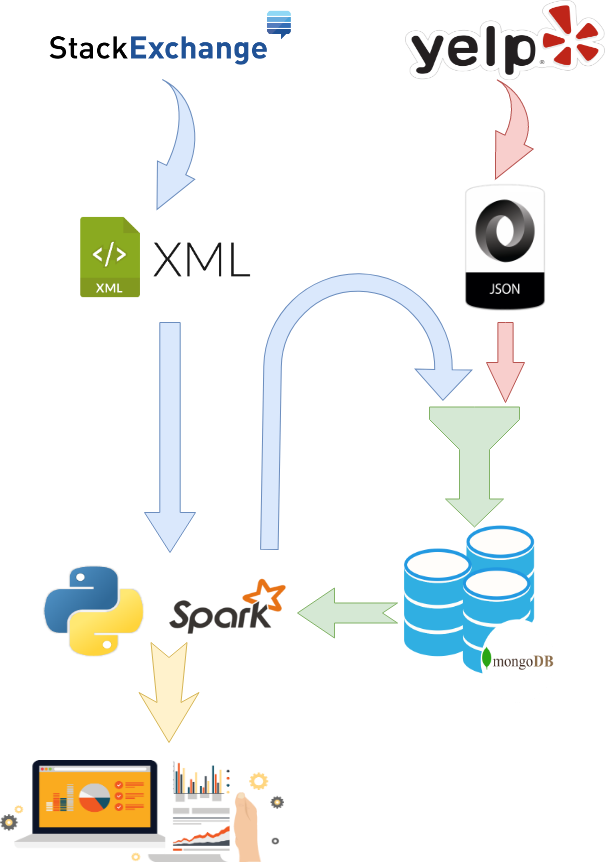
\includegraphics[scale=0.5]{image/BDABI.png}
	\caption{Architettura}
	\label{fig:arc}
\end{figure}
\section{JSON a MongoDB}
I file JSON di Yelp sono stati caricati direttamente in MongoDB grazie al JSON parser offerto.
Per il caricamento, ad esempio, delle recensioni, si è potuto adoperare il comando in \textbf{\ref{lst:mimp}}. Esso indica in quale database ed in quale collezione caricare i dati.\par

\begin{lstlisting}[language=Bash, caption={Yelp Dataset Loading}, captionpos=b, label={lst:mimp}]
mongoimport --db BDABI --collection yelpreview --file review.json
\end{lstlisting}

\section{XML a MongoDB}
Per i file XML, invece, MongoDB non offre delle estensioni per la conversione in BSON. Per il caricamento dei file di StackExchange, quindi, è stato adoperato Pyspark. Il codice prevede la creazione di una sessione Spark e la definizione degli schemi XML. Segue la creazione dei \emph{DataFrame} a partire dai file XML. La definizione dello schema non è strettamente necessaria per il caricamento: Spark potrebbe effettuare l'analisi dell'intero dataset e ricavarne lo schema di conseguenza. Essa, quindi, mira a rendere efficiente l'elaborazione, dando a Spark indicazioni sullo schema da ricercare ed i tipi di attributi relativi, evitando l'analisi completa del dataset. Ciò si rivela cruciale quando si gestiscono grandi volumi di dati. Nel caso di StackExchange è richiesto che Spark elabori e carichi circa 60GB di file XML appartenenti ai diversi topic. Dopo la definizione dei DataFrame, segue la scrittura in MongoDB degli stessi. La collezione in cui scrivere i dati è determinata dal parametro di ingresso alla funzione, rappresentante il topic. In tal modo i dati di StackExchange sono già differenziati per topic e sarà semplice un recupero in tal senso nella fase finale di analisi.
\begin{lstlisting}[language=Python, caption={StackExchange Dataset Loading}, captionpos=b,label={lst:se}]
#coding=utf-8
from pyspark.sql import SparkSession
from pyspark.sql.types import *
import sys

#Funzione con parametro di ingresso: sys.argv[1] = topic

database = "BDABI"
collectionpost = "stackexchange"+sys.argv[1]+"post"
collectionuser = "stackexchange"+sys.argv[1]+"user"

#Configurazione SparkSession e connessione con MongoDB
spark = SparkSession.builder.appName("stackExchange")
	.config("spark.mongodb.input.uri",
		"mongodb://127.0.0.1/"+database+"."+collectionpost)
	.config("spark.mongodb.output.uri",
		"mongodb://127.0.0.1/"+database+"."+collectionpost)
	.getOrCreate()

#Schemi dei file XML
postSchema = StructType([StructField("_Id", StringType(), True), 
	StructField("_PostTypeId", StringType(), True), 
	StructField("_ParentId", StringType(), True), 
	StructField("_AcceptedAnswerId", StringType(), True), 
	StructField("_CreationDate", StringType(), True), 
	StructField("_Score", IntegerType(), True), 
	StructField("_ViewCount", IntegerType(), True), 
	StructField("_Body", StringType(),True), 
	StructField("_OwnerUserId", StringType(), True), 
	StructField("_LastEditorUserId", StringType(), True), 
	StructField("_LastEditorDisplayName", StringType(), True), 
	StructField("_LastEditDate", StringType(), True), 
	StructField("_LastActivityDate", StringType(), True), 
	StructField("_CommunityOwedDate", StringType(), True), 
	StructField("_ClosedDate", StringType(), True), 
	StructField("_Title", StringType(), True), 
	StructField("_Tags", StringType(), True), 
	StructField("_AnswerCount", IntegerType(), True), 
	StructField("_CommentCount", IntegerType(), True), 
	StructField("_FavoriteCount", IntegerType(), True), 
	StructField("_OwnerDisplayName", StringType(), True)])

userSchema = StructType([StructField("_Id", StringType(), True), 
	StructField("_Reputation", IntegerType(), True), 
	StructField("_CreationDate", StringType(), True), 
	StructField("_DisplayName", StringType(), True), 
	StructField("_AccountId", StringType(), True), 
	StructField("_LastAccessDate", StringType(),True), 
	StructField("_WebSiteUrl", StringType(), True), 
	StructField("_Location", StringType(), True), 
	StructField("_ProfileImageUrl", StringType(), True), 
	StructField("_AboutMe", StringType(), True), 
	StructField("_Views", IntegerType(), True), 
	StructField("_UpVotes", IntegerType(), True), 
	StructField("_DownVotes", IntegerType(), True), 
	StructField("_Age", IntegerType(), True), 
	StructField("EmailHash", StringType(), True)])

#Creazione DataFrame
post = spark.read.format('xml').options(rowTag='row')
	.load('/mnt/data/'+sys.argv[1]+'/Posts.xml',schema=postSchema)
	.withColumnRenamed("_Id","_postId")
user = spark.read.format('xml').options(rowTag='row')
	.load('/mnt/data/'+sys.argv[1]+'/Users.xml',schema=userSchema)
	.withColumnRenamed("_Id","_userId")

#Scrittura DataFrame in MongoDB
post.write.format("com.mongodb.spark.sql.DefaultSource")
	.mode("append")
	.save()
user.write.format("com.mongodb.spark.sql.DefaultSource")
	.mode("append")
	.option("database",database)
	.option("collection", collectionuser)
	.save()
\end{lstlisting}

La funzione di caricamento del dataset di StackExchange adopera per l'esecuzione i package messi a disposizione da Spark. In questo caso si rivela la potenza di Spark, che aumenta la produttività dello sviluppatore grazie alla sua interoperabilità con librerie di alto livello. In particolare sono stati utilizzati i package per la connessione mongo-spark e per l'analisi XML:

\begin{lstlisting}[language=Bash, caption={Spark Packages}, captionpos=b]
spark-submit --packages com.databricks:spark-xml_2.12:0.5.0,
	org.mongodb.spark:mongo-spark-connector_2.12:2.4.0 
	/home/vmadmin/src/StackExchange.py topic
\end{lstlisting}

\section{Expert Finding}
MongoDB sarà ora pronto per fornire i dati per le elaborazioni successive. L'algoritmo, realizzato in Pyspark, si pone l'obiettivo di ricercare gli utenti esperti in un determinato argomento. Ricevuto in input il topic di riferimento, l'algoritmo effettua una ricerca nei diversi dataset e recupera i \emph{top10} utenti che valuta come esperti. La valutazione della competenza degli utenti è effettuata mediante una metrica che si avvale di diversi parametri offerti dai dataset.\par
L'algoritmo, in prima battuta, trasforma il topic in input nella forma coerente con i diversi dataset. Essi, infatti, memorizzano i topic con formati diversi e questa eterogeneità è gestita a monte in tal modo: Yelp richiede una stringa in minuscolo con la prima lettera in maiuscolo ed uno spazio tra le diverse parole, StackExchange richiede una stringa tutta in minuscolo senza spazi tra le parole. Dopo la fase di trasformazione, segue la ricerca.\par 
In Yelp si recuperano tutte le imprese appartenenti alla categoria ricercata e si sfruttano i loro id per trovare le recensioni degli utenti relativi mediante l'operazione di \emph{join} offerta da Spark. Ad ogni recensione è associata un'informazione di utilità valutata dai lettori. Si filtrano, quindi, le recensioni con utilità maggiore della media e si ordinano in ordine decrescente per utilità. Si selezionano le 100 recensioni più utili. Infatti l'algoritmo restituirà i 10 utenti più esperti e sarebbe dispendioso continuare l'elaborazione considerando un numero di recensioni superiore di più di un ordine di grandezza rispetto al numero di utenti cercati. Tra le recensioni più utili si devono determinare gli utenti più esperti. Si procede, quindi, ad un ulteriore join con gli utenti. Si raggruppano le recensioni per utente e si somma l'utilità di quelle afferenti allo stesso utente, creando l'attributo di \textbf{topicuseful}. Esso rappresenta la somma comulativa delle recensioni scritte da uno stesso utente relative al topic di riferimento. Le recensioni utili da sole non bastano ad identificare un utente esperto. Si è preso in considerazione il concetto di credibilità dell'utente, di autorità. Si reputa, infatti, esperto in un dato argomento un individuo che mostra padronanza della materia non solo in un caso isolato.  Per fare ciò si sono prese in considerazione differenti informazioni circa l'utente:
\begin{itemize}
\item il numero di anni in cui è stato un utente elite (selezionato dalla piattaforma come competente),
\item il numero di complimenti per le sue recensioni,
\item la somma cumulativa dell'utilità delle sue recensioni,
\item il numero di complimenti sul suo profilo,
\item il numero di fan,
\item il numero di complimenti per la lista di imprese recensite.
\end{itemize}
Si è definita, dunque, una metrica per ricavare una valutazione della competenza dell'utente a partire da queste informazioni. Per renderle omogenee, esse sono state normalizzate nel range [0,1]:
\begin{equation*}
x_{normalizzato} = \frac{x - min(x)}{max(x)-min(x)}
\end{equation*}
Si è poi definita la metrica di valutazione della competenza come somma pesata di questi attributi normalizzati:
\begin{equation*}
\sum_{1}^{7}{w_i*x_{{normalizato}_i}}
\end{equation*}
\begin{equation*}
w_i=\begin{cases} 0.25, & \mbox{se } x_i \in \mbox{ \{topicuseful, elitedim\}}\\ 0.15, & \mbox{se } x_i \in \mbox{ \{compliment hot\}}\\ 0.1, & \mbox{se } x_i \in \mbox{ \{fans, compliment profile, useruseful\}} \\ 0.05, & \mbox{se } x_i \in \mbox{ \{compliment list\}}
\end{cases}
\end{equation*}
Si ricavano infine i 10 utenti con score più alto.\par
In StackExchange i dati già sono divisi per topic. Si accede, quindi, con l'argomento in ingresso alla collezione corrispondente di MongoDB. Si ricavano i post relativi all'argomento, si filtrano solo quelli di risposta. Segue un ulteriore filtraggio in base allo score associato al post: si mantengono tutti i post con score maggiore della media, disposti poi in ordine decrescente. Ancora una volta, si limitano i post ai migliori 100 per le considerazioni fatte precedentemente. Si passa di seguito alla ricerca degli esperti. Si accede alla collezione degli utenti e, mediante inner join, si ricavano gli utenti relativi ai migliori post trovati. Segue il raggruppamento dei post sugli utenti, per ciascuno dei quali viene calcolata la somma degli score dei suoi post relativi al topic di riferimento. Questo attributo viene combinato alla reputazione dell'utente per calcolare la valutazione di competenza. La reputazione dell'utente è un'informazione sintetica che calcola StackExchange in base agli apprezzamenti ed alla storia dell'utente. Viene sfruttata per determinare l'autorevolezza dell'opinione dell'utente. Si definisce nuovamente la metrica per la valutazione della competenza sfruttando la normalizzazione degli attributi e dando a ciascuno di essi un peso del 50\%.

\begin{equation*}
\sum_{1}^{2}{0.5*x_{{normalizato}_i}}
\end{equation*}

\begin{equation*}
    x_i \in \{\mbox{topicscore, reputation}\}
\end{equation*}

\begin{lstlisting}[language=Python, caption={Expert Finding}, captionpos=b, label={lst:ef}]
# encoding=utf8
import sys
reload(sys)
sys.setdefaultencoding('utf8')
from pyspark.sql import SparkSession
from pyspark.sql.functions import col, avg, length, min, max, sum
import sys

#Creazione della sessione Spark con relativa configurazione 
#(wrapper di SparkContext)
spark = SparkSession.builder.appName("ExpertFinding")
	.config("spark.mongodb.input.uri", 
	"mongodb://127.0.0.1/BDABI.yelpbusiness")
	.getOrCreate()

#Valutazione degli argomenti di input:
#       - nessun argomento di input --> Topic non selezionato
#       - almeno un argomento di input --> Creazione della stringa 
#					corrispondente al topic da 
#					cercare in MongoDB
if len(sys.argv)>1:
  topicstack = ""
  for i in range(1,len(sys.argv)):
    line = sys.argv[i].capitalize()     #argomento in input tutto 
#				minuscolo con prima lettera maiuscola
    linestack = sys.argv[i].lower()
    if i==1:
      topic = line
    else:
      topic = topic+" "+line            #spazio tra piu' parole dello stesso 
#					topic
    topicstack = topicstack+linestack
  print ("Topic selezionato: %s") %topic

  collectionpost = "stackexchange"+topicstack+"post"
  collectionuser = "stackexchange"+topicstack+"user"
  notyelp = False
  notstack = False

#Normalizzazione in (0,1): (x-min)/(max-min)
  def normalizza(df,cl):
    minimo = df.agg(min(cl)).collect()[0][0]
    massimo = df.agg(max(cl)).collect()[0][0]
    return((df[cl]-minimo)/(massimo-minimo))


#Lettura dalla collezione yelpbusiness di MongoDB
  business = spark.read.format("com.mongodb.spark.sql.DefaultSource")
	.load()

#Ricerca in business dei locali relativi al topic selezionato
  category = business.where(col('categories').like(topic+",%") 
	| col('categories').like("% "+topic+",%") 
	| col('categories').like("% "+topic) 
	| col('categories').like(topic))
	.select("business_id")

#Lettura della collezione post di stackexchange
  post = spark.read.format("com.mongodb.spark.sql.DefaultSource")
	.option("uri","mongodb://127.0.0.1/BDABI."+collectionpost)
	.load()

  if category.count()>0:
    print("YELP")
#Lettura dalla collezione yelpreview di MongoDB
    review = spark.read.format("com.mongodb.spark.sql.DefaultSource")
    	.option("uri","mongodb://127.0.0.1/BDABI.yelpreview")
    	.load()
#Selezione delle colonne di interesse di review
    reviewsel = review.select('business_id', 'user_id', 'useful')
#Join per la ricerca delle recensioni appartenenti ai locali 
#precedentemente trovati
    reviewtopic = category.join(reviewsel,
    	category.business_id==reviewsel.business_id, "inner")
    	.select('user_id', 'useful')
#Filtraggio delle recensioni con utilita' inferiore alla media 
#ed ordinamento discendente
    reviewfilt = reviewtopic
    	.filter(reviewtopic['useful'] > 
    		reviewtopic.agg(avg(col("useful"))).collect()[0][0])
    	.orderBy('useful', ascending=False)
    if reviewfilt.count()>100:
      reviewfilt = reviewfilt.limit(100)        #riduzione a 100 righe 
      #						con maggiore useful

#Lettura della collezione yelpuser di MongoDB
    user = spark.read.format("com.mongodb.spark.sql.DefaultSource")
    	.option("uri","mongodb://127.0.0.1/BDABI.yelpuser")
    	.load()
    usersel = user
    	.select('user_id','name','useful','fans','elite',
    		'compliment_hot','compliment_profile',
    		'compliment_list')
    	.withColumnRenamed("useful","useruseful")

#Join recensioni-utenti, calcolo della dimensione di elite, 
#selezione colonne di interesse e somma di useful delle recensioni 
#afferenti allo stesso utente
#La dimensione di elite e' la lunghezza della stringa
    reviewer = reviewfilt.join(usersel, 
    		reviewfilt.user_id==usersel.user_id, "inner")
    	.withColumn('elitedim',length('elite'))
    	.groupBy('name','useruseful','fans','elitedim',
    		'compliment_hot','compliment_profile',
    		'compliment_list',usersel.user_id)
    	.agg({'useful':'sum'})
    	.withColumnRenamed("sum(useful)","topicuseful")

#Calcolo score di ogni utente
#Gli attributi contribuiscono con peso differente al calcolo 
#dello score: 5% list, 10% fans, useruseful e profile, 15% hot, 
#25% elite e topicuseful
    userscore = reviewer.withColumn('score', 
	    	(0.25*normalizza(reviewer,'topicuseful'))+
	    	(0.1*normalizza(reviewer,'fans'))+
	    	(0.25*normalizza(reviewer,'elitedim'))+
	    	(0.15*normalizza(reviewer,'compliment_hot'))+
	    	(0.1*normalizza(reviewer,'compliment_profile'))+
	    	(0.05*normalizza(reviewer,'compliment_list'))+
	    	(0.1*normalizza(reviewer,'useruseful')))
    	.select('user_id','name','score')
    	.orderBy('score',ascending=False)
    userscore.show(10)
  else:
    notyelp = True

  if post.count()>0:
    print("STACK EXCHANGE")
    postsel = post.filter(post['_PostTypeId']=="2")
    	.select("_postId","_Score","_OwnerUserId")
    	.filter(post['_Score'] > 
    		post.agg(avg(col("_Score"))).collect()[0][0])
    	.orderBy('_Score', ascending=False)

    if postsel.count()>100:
      postsel = postsel.limit(100)       #riduzione a 100 righe con 
#						maggiore score

#Lettura della collezione user di stackexchange
    user = spark.read.format("com.mongodb.spark.sql.DefaultSource")
	.option("uri","mongodb://127.0.0.1/BDABI."+collectionuser)
	.load()
    usersel = user.select('_userId','_DisplayName','_Location',
    	'_AboutMe','_Reputation')

#Join post-utenti, selezione colonne di interesse e somma di
# score dei post afferenti allo stesso utente
    expert = postsel.join(usersel, 
    		postsel['_OwnerUserId']==usersel['_userId'], "inner")
    	.groupBy('_userId','_DisplayName','_Location','_AboutMe',
    		'_Reputation')
    	.agg({'_Score':'sum'})
    	.withColumnRenamed("sum(_Score)","topicscore")

#Calcolo dello score di ogni utente
    expertscore = expert.withColumn('scoreexpertise', 
    		(0.5*normalizza(expert,'topicscore'))+
    		(0.5*normalizza(expert,'_Reputation')))
    	.orderBy('scoreexpertise',ascending=False)
    expertscore.show(10)
    expertscore.select('_DisplayName','_AboutMe').show(10,False)

  else:
    notstack = True

  if (notyelp and notstack):
    print("Topic inesistente")

else:
  print("Topic non selezionato")
\end{lstlisting}

\begin{algorithm}[ht]
	\caption{Expert Finding Pseudocode}
	\KwIn{topic}
	\KwResult{experts}
	\eIf{topic composto da almeno una parola}{	
		Trasformazione topic in parole staccate, minuscole e con la prima lettera maiuscola per Yelp\;
		Trasformazione topic in parole unite e minuscole per StackExchange\;
		notYelp = False; notStack = False\;
		Recupero da MongoDB le imprese di Yelp con categoria == topic\;
		Recupero da MongoDB i post di StackExchange appartenenti alla collezione di topic\;
		\eIf{numero imprese > 0}{
			Recupero da MongoDB le recensioni di Yelp e selezione degli attributi di interesse\;
			Recupero delle recensioni relative alle imprese\;
			Filtraggio recensioni con utilità > media(utilità)\;
			Riduzione ad almeno le 100 recensioni più utili\;
			Recupero da MongoDB gli utenti di Yelp e selezione degli attributi di interesse\;
			Recupero degli utenti autori delle recensioni più utili\;
			Raggruppamento delle recensioni per utente e somma dell'utilità delle recensioni di uno stesso utente\;
			Calcolo competenza come somma pesata degli attributi più importanti normalizzati\;
			Ordinamento decrescente per competenza e selezione dei primi 10 utenti\;
		}{notYelp = True}
		\eIf{numero post > 0}{
			Filtraggio dei post di risposta e selezione degli attributi di interesse\;
			Filtraggio dei post con score > media(score)\;
			Riduzione ad almeno i 100 post con score più alto\;
			Recupero da MongoDB gli utenti di StackExchange appartenenti alla collezione di topic e selezione degli attributi di interesse\;
			Recupero degli utenti autori dei migliori post\;
			Raggruppamento dei post per utente e somma dello score dei post di uno stesso utente\;
			Calcolo competenza come somma pesata degli attributi più importanti normalizzati\;
			Ordinamento decrescente per competenza e selezione dei primi 10 utenti\;
		}{notStack = True}
		
		\If{notYelp AND notStack}{print "Topic inesistente"\;}
	}{print "Topic non selezionato"\;}
\end{algorithm}

Infine, per eseguire il codice Python, si sfrutta Spark con il package mongo-spark-connector. Per garantire l'esecuzione è necessario fornire sufficiente memoria per il driver, pena il fallimento dell'esecuzione. Sono stati dedicati al driver 2GB di memoria centrale. L'output è direzionato verso un file testo per distinguerlo dalle informazioni di controllo dell'esecuzione.

\begin{lstlisting}[language=Bash, caption={Driver Memory}, captionpos=b,label={lst:dm}]
spark-submit 
--packages org.mongodb.spark:mongo-spark-connector_2.12:2.4.0 
--driver-memory 2g 
/home/vmadmin/src/ExpertFinding.py topic >risultato.txt
\end{lstlisting}
	\chapter{Risultati sperimentali}
Attraverso i comandi del tipo in \textbf{Figura \ref{lst:mimp}} sono stati caricati i file JSON nel database BDABI di MongoDB nella collezione \emph{yelp}+nomefile. Attraverso il codice in \textbf{Figura \ref{lst:se}} sono stati caricati i file XML nel database BDABI di MongoDB nella collezione \emph{stackexchange}+topic+nomefile. Al seguito di questa fase di caricamento, rendiamo operativo MongoDB per le successive elaborazioni. In \textbf{Figura \ref{fig:mongo}} osserviamo alcune delle centinaia collezioni caricate.

\begin{figure}[H]
	\centering
	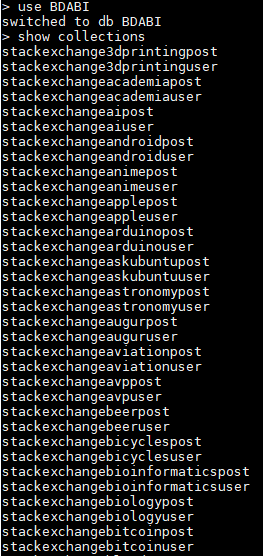
\includegraphics[scale=0.9]{image/mongo1.PNG}
	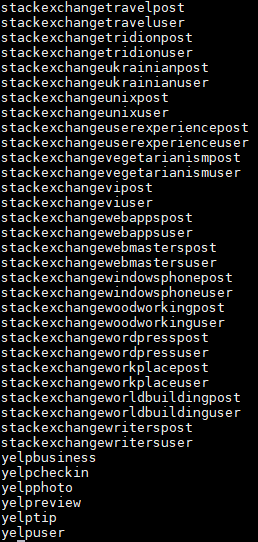
\includegraphics[scale=0.9]{image/mongo2.PNG}
	\caption{MongoDB}
	\label{fig:mongo}
\end{figure}

Conclusasi questa fase, non resta che sfruttare i dati che si dispone per effettuare la ricerca degli esperti su di un determinato argomento. Ricerchiamo gli esperti di \emph{Golf}. Lanciamo il comando in \textbf{Figura \ref{lst:dm}} con golf come topic. Osserviamo un tempo di elaborazione di poco più di 12 minuti. Essa ha coinvolto principalmente il dataset di Yelp, grazie alle recensioni sui campi da golf. Si ottengono gli esperti relativi.

\begin{figure}[H]
	\centering
	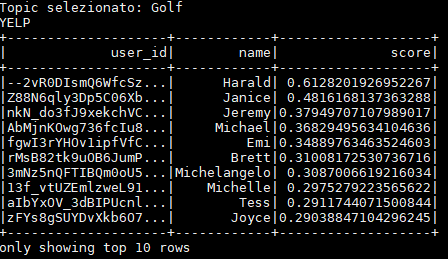
\includegraphics{image/golf.PNG}
	\caption{Esperti di golf}
	\label{fig:golf}
\end{figure}

Analogamente effettuiamo un'ulteriore ricerca di esperti di animali. Osserviamo che il tempo di esecuzione è poco più di 12 minuti. La ricerca è stata effettuata su entrambi i dataset. Risulta interessante osservare le descrizioni che hanno dato gli utenti di loro stessi. La maggior parte di esse fanno riferimento ad un aspetto della vita dell'utente correlato agli animali. Sono dunque persone che reputano il loro rapporto con gli animali come una delle cose primarie da inserire in una descrizione personale.

\begin{description}
	\item[Zaralynda]Avid reader, feminist, owned by cats, sometime gamer, and quilter.
	Currently share my home with 3 cats.
	\item[Yvette Colomb]Animal lover and animal rights activist.
	\item[Trond Hansen]I am 53 years old (young). My interests are very broad: science, astronomy, biology, geology, marine biology. I simply want to know how every thing works, I have a cat named Trine. I have always had a cat.
	\item[Rebecca RVT]Graduated as Veterinary Technician in spring 2013, got certified in summer of 2013. Currently work primarily with  animal (cats and dogs). I have 11 years experience with exotic pets (pocket pets, reptiles and birds) with 2 years of working at an exotic pet practice.
	\item[James Jenkins]I volunteer with \url{http://www.petfinder.com/shelters/PA323.html} Rabbit Wranglers. I can often be found at local community events walking a rabbit on a leash, providing education and offering tips for adopting and rating a pet house rabbit into the family.
	
\end{description}

\begin{figure}[H]
	\centering
	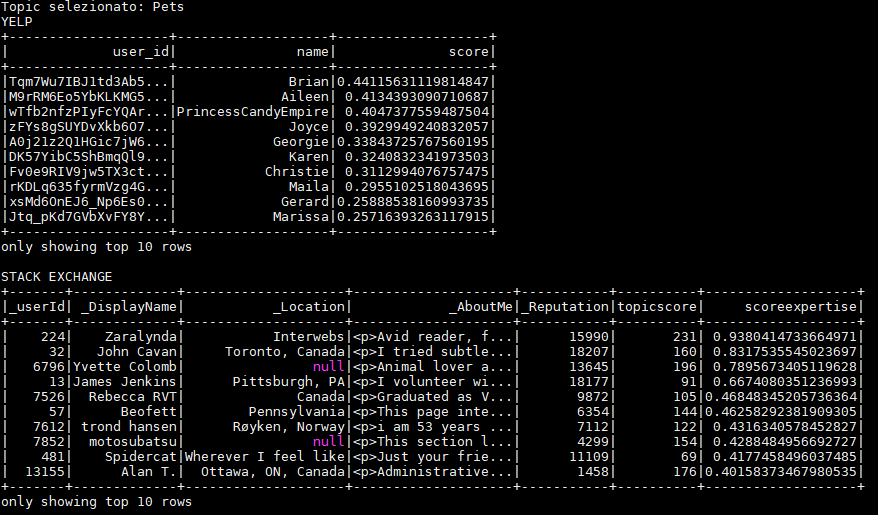
\includegraphics[scale=0.7]{image/pets.PNG}
	\caption{Esperti di animali}
	\label{fig:pets}
\end{figure}
\begin{figure}[H]
	\centering
	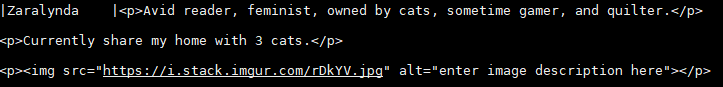
\includegraphics[scale=0.8]{image/pets2.PNG}
	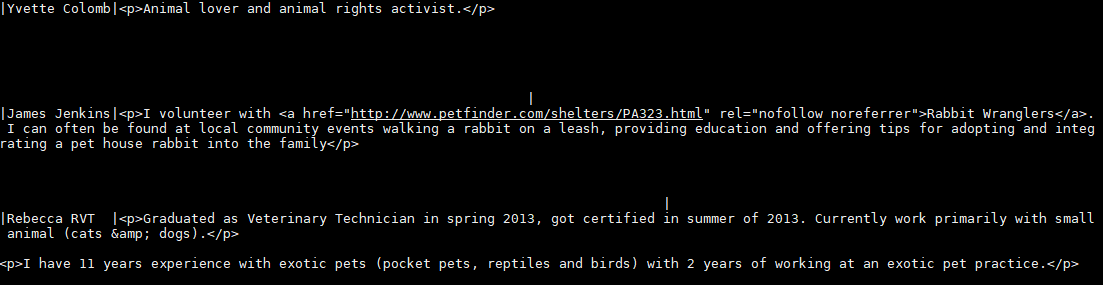
\includegraphics[width=16cm]{image/pets3.PNG}
	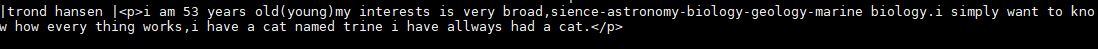
\includegraphics[width=16cm]{image/pets4.PNG}
	\caption{About Me degli esperti di animali}
	\label{fig:abme}
\end{figure}

Infine ricerchiamo gli esperti di informatica. L'esecuzione impiega 30 secondi e coinvolge solo il dataset di StackExchange. Osserviamo ancora una volta come le descrizioni degli utenti siano coerenti con la tipologia di esperto cercata: un ricercatore del Technion, un ingegnere del software di Google, un dottorando dell'Università di British Columbia, un professore dell'Università dell'Illinois.

\begin{description}
	\item[Yuval Filmus]Assistant Professor in the Department of Computer Science at the Technion.
	\item[Raphael]I am a computer scientist by training, which means I now think like one: always analysing,  abstracting, reducing, problem solving. In addition, I picked up some affection and, hopefully, ability for actually building software over the years. You can take a look over on \url{https://github.com/reitzig} Github. During my time at university I have found a passion for teaching, by which I mean helping people learn. Some say I was quite the nitpicker; it's for your best, I promise! In my free time I play games, read books, code, work out, enjoy music, and roam the webs.
	\item[Kaveh]\url{http://ca.linkedin.com/in/ghasemloo} Software Engineer at \url{http://www.google.com} Google. Ph.D. in Computer Science, \url{https://www.utoronto.ca/} University of Toronto, \url{http://web.cs.toronto.edu/} Department of Computer Science, \url{http://www.cs.toronto.edu/theory/index.php} Theory Group. Thesis: \url{http://www.cs.toronto.edu/~kaveh/papers/phd-thesis.pdf} "Uniformity and Nonuniformity in Proof Complexity", 2016. Ex-moderator on \url{http://cstheory.stackexchange.com} cstheory.
	\item[Jmite]I am Joey Eremondi, a PhD Student at the \url{https://www.cs.ubc.ca/} University of British Columbia. I do research in Programming Languages and Theory of Computation, particularly with dependent types. My \url{http://dspace.library.uu.nl/handle/1874/337692} Masters Thesis was on improving error messages for higher order unification. I've also co-authored a few papers on reversal-bounded counter automata. I have an M.Sc in Computing Science from \url{http://www.cs.uu.nl/} Utrecht University, a B.Sc. Honours in Computer Science, and a B.Sc. 4-year in Mathematics, both from the \url{http://www.usask.ca/" rel=} University of Saskatchewan.
	\item[JeffE]I am a full professor of \url{http://www.cs.uiuc.edu} computer science at the University of Illinois, Urbana-Champaign.  I teach \url{http://www.cs.uiuc.edu/~jeffe/teaching/algorithms} algorithms.
	
\end{description}

\begin{figure}[H]
	\centering
	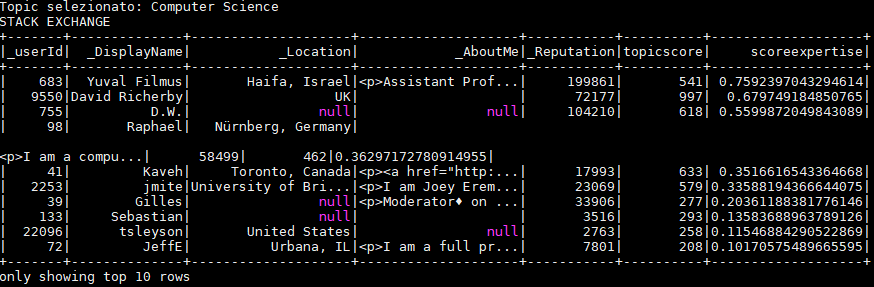
\includegraphics[scale=0.7]{image/cs.PNG}
	\caption{Esperti di informatica}
	\label{fig:cs}
\end{figure}

La metrica di valutazione della competenza riesce efficacemente ad individuare gli esperti nel settore. Le differenze sostanziali nei tempi di elaborazione sono dovute alla composizione dei dataset. Essendo StackExchange già suddiviso per topic, presenterà un numero di tuple nettamente inferiore alle centinaia di migliaia di Yelp, che mantiene i dati di tutta la piattaforma senza scrematura. La composizione di Yelp necessita inoltre di un'operazione di Join aggiuntiva per ricavare i topic dalle aziende, e di conseguenza le recensioni relative. Differenti configurazioni tecniche di Spark, variando il numero di esecutori, di core per ciascuno di essi, e di memoria loro disponibile, possono portare ad una riduzione dei tempi globali di al più 10 secondi, suggerendo che non siano le limitazioni tecniche della piattaforma a vincolare eccesivamente i tempi.
	
\end{document}